% Options for packages loaded elsewhere
\PassOptionsToPackage{unicode}{hyperref}
\PassOptionsToPackage{hyphens}{url}
%
\documentclass[
]{article}
\usepackage{lmodern}
\usepackage{amssymb,amsmath}
\usepackage{ifxetex,ifluatex}
\ifnum 0\ifxetex 1\fi\ifluatex 1\fi=0 % if pdftex
  \usepackage[T1]{fontenc}
  \usepackage[utf8]{inputenc}
  \usepackage{textcomp} % provide euro and other symbols
\else % if luatex or xetex
  \usepackage{unicode-math}
  \defaultfontfeatures{Scale=MatchLowercase}
  \defaultfontfeatures[\rmfamily]{Ligatures=TeX,Scale=1}
\fi
% Use upquote if available, for straight quotes in verbatim environments
\IfFileExists{upquote.sty}{\usepackage{upquote}}{}
\IfFileExists{microtype.sty}{% use microtype if available
  \usepackage[]{microtype}
  \UseMicrotypeSet[protrusion]{basicmath} % disable protrusion for tt fonts
}{}
\makeatletter
\@ifundefined{KOMAClassName}{% if non-KOMA class
  \IfFileExists{parskip.sty}{%
    \usepackage{parskip}
  }{% else
    \setlength{\parindent}{0pt}
    \setlength{\parskip}{6pt plus 2pt minus 1pt}}
}{% if KOMA class
  \KOMAoptions{parskip=half}}
\makeatother
\usepackage{xcolor}
\IfFileExists{xurl.sty}{\usepackage{xurl}}{} % add URL line breaks if available
\IfFileExists{bookmark.sty}{\usepackage{bookmark}}{\usepackage{hyperref}}
\hypersetup{
  pdftitle={Chaffinches (again)},
  pdfauthor={Hannah Clark},
  hidelinks,
  pdfcreator={LaTeX via pandoc}}
\urlstyle{same} % disable monospaced font for URLs
\usepackage[margin=1in]{geometry}
\usepackage{color}
\usepackage{fancyvrb}
\newcommand{\VerbBar}{|}
\newcommand{\VERB}{\Verb[commandchars=\\\{\}]}
\DefineVerbatimEnvironment{Highlighting}{Verbatim}{commandchars=\\\{\}}
% Add ',fontsize=\small' for more characters per line
\usepackage{framed}
\definecolor{shadecolor}{RGB}{248,248,248}
\newenvironment{Shaded}{\begin{snugshade}}{\end{snugshade}}
\newcommand{\AlertTok}[1]{\textcolor[rgb]{0.94,0.16,0.16}{#1}}
\newcommand{\AnnotationTok}[1]{\textcolor[rgb]{0.56,0.35,0.01}{\textbf{\textit{#1}}}}
\newcommand{\AttributeTok}[1]{\textcolor[rgb]{0.77,0.63,0.00}{#1}}
\newcommand{\BaseNTok}[1]{\textcolor[rgb]{0.00,0.00,0.81}{#1}}
\newcommand{\BuiltInTok}[1]{#1}
\newcommand{\CharTok}[1]{\textcolor[rgb]{0.31,0.60,0.02}{#1}}
\newcommand{\CommentTok}[1]{\textcolor[rgb]{0.56,0.35,0.01}{\textit{#1}}}
\newcommand{\CommentVarTok}[1]{\textcolor[rgb]{0.56,0.35,0.01}{\textbf{\textit{#1}}}}
\newcommand{\ConstantTok}[1]{\textcolor[rgb]{0.00,0.00,0.00}{#1}}
\newcommand{\ControlFlowTok}[1]{\textcolor[rgb]{0.13,0.29,0.53}{\textbf{#1}}}
\newcommand{\DataTypeTok}[1]{\textcolor[rgb]{0.13,0.29,0.53}{#1}}
\newcommand{\DecValTok}[1]{\textcolor[rgb]{0.00,0.00,0.81}{#1}}
\newcommand{\DocumentationTok}[1]{\textcolor[rgb]{0.56,0.35,0.01}{\textbf{\textit{#1}}}}
\newcommand{\ErrorTok}[1]{\textcolor[rgb]{0.64,0.00,0.00}{\textbf{#1}}}
\newcommand{\ExtensionTok}[1]{#1}
\newcommand{\FloatTok}[1]{\textcolor[rgb]{0.00,0.00,0.81}{#1}}
\newcommand{\FunctionTok}[1]{\textcolor[rgb]{0.00,0.00,0.00}{#1}}
\newcommand{\ImportTok}[1]{#1}
\newcommand{\InformationTok}[1]{\textcolor[rgb]{0.56,0.35,0.01}{\textbf{\textit{#1}}}}
\newcommand{\KeywordTok}[1]{\textcolor[rgb]{0.13,0.29,0.53}{\textbf{#1}}}
\newcommand{\NormalTok}[1]{#1}
\newcommand{\OperatorTok}[1]{\textcolor[rgb]{0.81,0.36,0.00}{\textbf{#1}}}
\newcommand{\OtherTok}[1]{\textcolor[rgb]{0.56,0.35,0.01}{#1}}
\newcommand{\PreprocessorTok}[1]{\textcolor[rgb]{0.56,0.35,0.01}{\textit{#1}}}
\newcommand{\RegionMarkerTok}[1]{#1}
\newcommand{\SpecialCharTok}[1]{\textcolor[rgb]{0.00,0.00,0.00}{#1}}
\newcommand{\SpecialStringTok}[1]{\textcolor[rgb]{0.31,0.60,0.02}{#1}}
\newcommand{\StringTok}[1]{\textcolor[rgb]{0.31,0.60,0.02}{#1}}
\newcommand{\VariableTok}[1]{\textcolor[rgb]{0.00,0.00,0.00}{#1}}
\newcommand{\VerbatimStringTok}[1]{\textcolor[rgb]{0.31,0.60,0.02}{#1}}
\newcommand{\WarningTok}[1]{\textcolor[rgb]{0.56,0.35,0.01}{\textbf{\textit{#1}}}}
\usepackage{longtable,booktabs}
% Correct order of tables after \paragraph or \subparagraph
\usepackage{etoolbox}
\makeatletter
\patchcmd\longtable{\par}{\if@noskipsec\mbox{}\fi\par}{}{}
\makeatother
% Allow footnotes in longtable head/foot
\IfFileExists{footnotehyper.sty}{\usepackage{footnotehyper}}{\usepackage{footnote}}
\makesavenoteenv{longtable}
\usepackage{graphicx,grffile}
\makeatletter
\def\maxwidth{\ifdim\Gin@nat@width>\linewidth\linewidth\else\Gin@nat@width\fi}
\def\maxheight{\ifdim\Gin@nat@height>\textheight\textheight\else\Gin@nat@height\fi}
\makeatother
% Scale images if necessary, so that they will not overflow the page
% margins by default, and it is still possible to overwrite the defaults
% using explicit options in \includegraphics[width, height, ...]{}
\setkeys{Gin}{width=\maxwidth,height=\maxheight,keepaspectratio}
% Set default figure placement to htbp
\makeatletter
\def\fps@figure{htbp}
\makeatother
\setlength{\emergencystretch}{3em} % prevent overfull lines
\providecommand{\tightlist}{%
  \setlength{\itemsep}{0pt}\setlength{\parskip}{0pt}}
\setcounter{secnumdepth}{5}
\usepackage{booktabs}
\usepackage{longtable}
\usepackage{array}
\usepackage{multirow}
\usepackage{wrapfig}
\usepackage{float}
\usepackage{colortbl}
\usepackage{pdflscape}
\usepackage{tabu}
\usepackage{threeparttable}
\usepackage{threeparttablex}
\usepackage[normalem]{ulem}
\usepackage{makecell}
\usepackage{xcolor}

\title{Chaffinches \emph{(again)}}
\author{Hannah Clark}
\date{04/11/2020}

\begin{document}
\maketitle

{
\setcounter{tocdepth}{2}
\tableofcontents
}
\hypertarget{introduction}{%
\subsection{Introduction}\label{introduction}}

Chaffinches, \emph{Fringilla coelebs}, are common to UK woodland, farmland, parks, and gardens (Woodland Trust, n.d.). The average weight of a chaffinch is 18-29g (RSPB, n.d.). The masses of a group of finches were taken and categorised by sex, to see how this varied from this known average. See Figure \ref{fig:malechaff-fig}



\begin{figure}
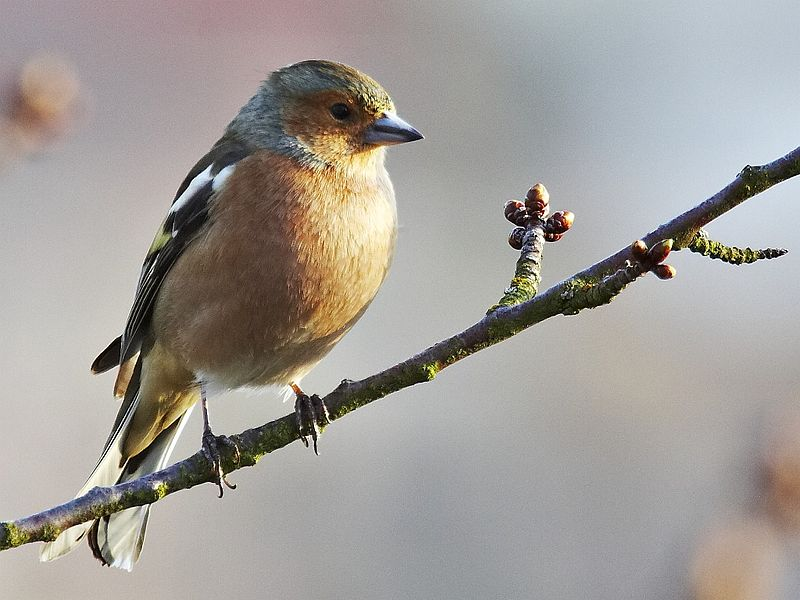
\includegraphics[height=200px]{figures/malechaff01} \caption{A male chaffinch. Photo taken by Michael Apel, CC BY 2.5, \url{https://en.wikipedia.org/wiki/Common_chaffinch\#/media/File:Fringilla_coelebs_male1.jpg}}\label{fig:malechaff-fig}
\end{figure}

\hypertarget{methods}{%
\subsection{Methods}\label{methods}}

The chaffinches data was imported and tidied

\begin{Shaded}
\begin{Highlighting}[]
\CommentTok{#read in the data}
\NormalTok{chaff <-}\StringTok{ }\KeywordTok{read.table}\NormalTok{(}\StringTok{"~/R Workshop/chaff02/data-raw/chaff.txt"}\NormalTok{, }\DataTypeTok{header =}\NormalTok{ T)}

\CommentTok{#tidying the data}
\NormalTok{chaff2 <-}\StringTok{ }\KeywordTok{gather}\NormalTok{(}\DataTypeTok{data =}\NormalTok{ chaff, }\DataTypeTok{key =}\NormalTok{ sex, }\DataTypeTok{value =}\NormalTok{ mass)}

\CommentTok{#write the tidied data into a new file}
\KeywordTok{write.table}\NormalTok{(chaff2, }\DataTypeTok{file =} \StringTok{'~/R Workshop/chaff02/data/tidychaff.txt'}\NormalTok{, }\DataTypeTok{row.names =} \OtherTok{FALSE}\NormalTok{)}
\end{Highlighting}
\end{Shaded}

Summarising the data

\begin{Shaded}
\begin{Highlighting}[]
\NormalTok{sum_sq <-}\StringTok{ }\ControlFlowTok{function}\NormalTok{(df, measure, group) \{}
\NormalTok{  df }\OperatorTok\StringTok{ }\KeywordTok{group_by}\NormalTok{(\{\{ group \}\}) }\OperatorTok\StringTok{ }
\StringTok{    }\KeywordTok{summarise}\NormalTok{(}\DataTypeTok{ss =} \KeywordTok{sum}\NormalTok{((\{\{measure\}\} }\OperatorTok{-}\StringTok{ }\KeywordTok{mean}\NormalTok{(\{\{measure\}\}))}\OperatorTok{^}\DecValTok{2}\NormalTok{))}
\NormalTok{\}}

\KeywordTok{sum_sq}\NormalTok{(chaff2, mass, sex)}
\end{Highlighting}
\end{Shaded}

\begin{verbatim}
## # A tibble: 2 x 2
##   sex        ss
##   <chr>   <dbl>
## 1 females  86.8
## 2 males    87.9
\end{verbatim}

\begin{Shaded}
\begin{Highlighting}[]
\NormalTok{chaff2 }\OperatorTok\StringTok{ }\KeywordTok{group_by}\NormalTok{(sex) }\OperatorTok\StringTok{ }
\StringTok{  }\KeywordTok{summarise}\NormalTok{(}\DataTypeTok{mean =} \KeywordTok{mean}\NormalTok{(mass),}
            \DataTypeTok{n =} \KeywordTok{length}\NormalTok{(n),}
            \DataTypeTok{sd =} \KeywordTok{sd}\NormalTok{(mass),}
            \DataTypeTok{se =}\NormalTok{ sd}\OperatorTok{/}\KeywordTok{sqrt}\NormalTok{(n))}
\end{Highlighting}
\end{Shaded}

\begin{verbatim}
## # A tibble: 2 x 5
##   sex      mean     n    sd    se
##   <chr>   <dbl> <int> <dbl> <dbl>
## 1 females  20.5     1  2.14  2.14
## 2 males    22.3     1  2.15  2.15
\end{verbatim}

This can also be done in 1 function

\begin{Shaded}
\begin{Highlighting}[]
\NormalTok{data_summary <-}\StringTok{ }\ControlFlowTok{function}\NormalTok{(df, measure, group) \{}
\NormalTok{  df }\OperatorTok\StringTok{ }\KeywordTok{group_by}\NormalTok{(\{\{ group \}\}) }\OperatorTok\StringTok{ }
\StringTok{    }\KeywordTok{summarise}\NormalTok{(}\DataTypeTok{mean =} \KeywordTok{mean}\NormalTok{(\{\{measure\}\}),}
            \DataTypeTok{n =} \KeywordTok{length}\NormalTok{(n),}
            \DataTypeTok{sd =} \KeywordTok{sd}\NormalTok{(\{\{measure\}\}),}
            \DataTypeTok{se =} \KeywordTok{sd}\NormalTok{(\{\{measure\}\})}\OperatorTok{/}\KeywordTok{sqrt}\NormalTok{(}\KeywordTok{length}\NormalTok{(n)),}
            \DataTypeTok{ss =} \KeywordTok{sum}\NormalTok{((\{\{measure\}\} }\OperatorTok{-}\StringTok{ }\KeywordTok{mean}\NormalTok{(\{\{measure\}\}))}\OperatorTok{^}\DecValTok{2}\NormalTok{))}
\NormalTok{\}}

\NormalTok{chaff3 <-}\StringTok{ }\KeywordTok{data_summary}\NormalTok{(chaff2, mass, sex)}
\end{Highlighting}
\end{Shaded}

\hypertarget{results}{%
\subsection{Results}\label{results}}

The results from summarising the chaffinches data, grouping by sex. See table @ref(tab: chaff-table)

\begin{table}

\caption{\label{tab:chaff-table}Chaffinch masses by sex}
\centering
\begin{tabular}[t]{l|r|r|r|r}
\hline
Sex & Mean mass & Standard deviation & Standard error & Sum squared\\
\hline
females & 20.48 & 2.14 & 2.14 & 86.83\\
\hline
males & 22.27 & 2.15 & 2.15 & 87.90\\
\hline
\end{tabular}
\end{table}

\hypertarget{discussion}{%
\subsection{Discussion}\label{discussion}}

\hypertarget{references}{%
\subsection*{References}\label{references}}
\addcontentsline{toc}{subsection}{References}

\hypertarget{refs}{}
\leavevmode\hypertarget{ref-noauthor_undated-dy}{}%
RSPB. n.d. ``Chaffinch.'' \url{https://www.rspb.org.uk/birds-and-wildlife/wildlife-guides/bird-a-z/chaffinch/}.

\leavevmode\hypertarget{ref-Woodland_Trust_undated-gv}{}%
Woodland Trust. n.d. ``Chaffinch.'' \url{https://www.woodlandtrust.org.uk/trees-woods-and-wildlife/animals/birds/chaffinch/}.

\end{document}
